\begin{figure*}[!t]
\centering
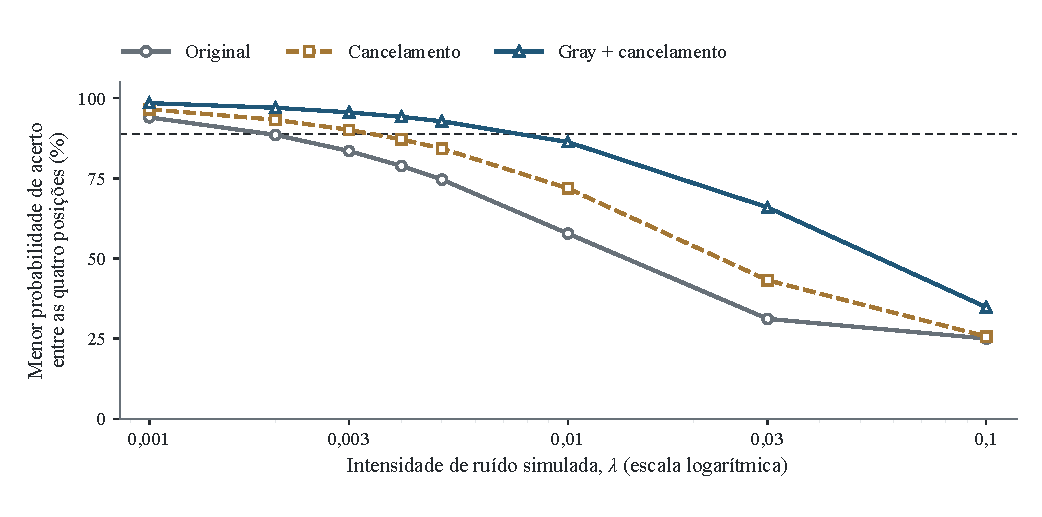
\includegraphics[width=\textwidth]{revisao-ruido.pdf}
\caption{Como o aumento do ruído afeta a busca na simulação. Cada ponto mostra o acerto da posição mais difícil entre as quatro testadas. O parâmetro $\lambda$ controla a intensidade do erro aplicado após operações CX; nas operações $U$, usa-se $\lambda/10$. A escala horizontal é logarítmica: distâncias iguais representam multiplicações, não somas iguais. Sem ruído, as três versões acertam 100\%; esse caso fica fora do eixo. As linhas unem valores testados. A linha tracejada indica os 88,89\% necessários para empatar com a referência clássica na contagem adotada.}
\label{fig:ruido}
\end{figure*}

\section{Resultados experimentais}
Os resultados respondem a duas perguntas diferentes. Primeiro, as contagens dos arquivos eleitorais concordam? Depois, quando introduzimos uma diferença conhecida em uma cópia, com que frequência Grover encontra a linha alterada? A primeira resposta vem da conferência nacional. A segunda vem das simulações e dos testes no computador da IBM.
\subsection{Reconferência nacional e controles}
Nas 499.207 seções examinadas, a contagem dos votos registrados coincidiu com o respectivo boletim. Esse conjunto inclui 499.178 boletins regulares e 29 do Sistema de Apuração, referentes a votos em cédulas. As somas também coincidiram com as tabelas publicadas e com os totais nacionais da Tabela~\ref{tab:nacional}.

A conferência abrangeu 1.931.103 linhas de votação presidencial, distribuídas por 499.205 seções com votos. Duas seções sem comparecimento completaram o conjunto apurado. Outras 41 não foram instaladas, completando o universo de 499.248 seções. Não foram encontradas diferenças de contagem, registros duplicados ou seções faltantes na comparação.

A verificação da assinatura digital do resultado nacional foi válida para a chave pública usada, e o conteúdo assinado coincidiu com o arquivo analisado. Uma cópia modificada falhou nessa verificação. O programa de comparação também detectou as quatro alterações introduzidas nas cópias de teste, inclusive a transferência de um voto entre categorias que mantinha a soma total. Isso mostra por que comparar apenas o total seria insuficiente. Os controles verificam esses erros específicos, sem cobrir todas as falhas possíveis.

\subsection{Execução inicial e revisão local}
A Tabela~\ref{tab:experimento} reúne os resultados iniciais. Sem erros simulados, as 12.288 medições devolveram a posição da diferença artificial. Com intensidade de ruído $\lambda=0{,}003$, o acerto caiu para 89,08\%. Seu intervalo de confiança, de 88,52\% a 89,62\%, inclui valores dos dois lados do limite de 88,89\%. Portanto, o resultado não permite afirmar economia de consultas com a confiança adotada. Com $\lambda=0{,}005$, a própria estimativa de acerto já está abaixo do limite.

Na execução inicial da IBM, a resposta correta era 01, o endereço da segunda linha. O computador devolveu 00 em 236 medições, 01 em 331, 10 em 384 e 11 em 1.097. Acertou, portanto, 16,16\%, com intervalo de 14,63\% a 17,82\%. Sortear uma das quatro linhas com chances iguais daria 25\% em média. A concentração de respostas em 11, que recebeu 53,56\% das medições, motivou as verificações posteriores. Essa execução isolada não identifica a causa do erro.

Na revisão local, passaram as 708 verificações da regra que marca as diferenças, distribuídas por 59 pares de tabelas e três versões do circuito. Sem ruído, a busca acertou 100\% em cada uma das quatro posições quando havia uma única divergência. Os casos com zero a quatro divergências reproduziram as probabilidades descritas na fundamentação teórica.

A Tabela~\ref{tab:variantes} compara as versões preparadas sob as mesmas condições. Com $\lambda=0{,}003$, o acerto da posição mais difícil foi 83,54\% na original, 90,16\% após retirar operações que se anulavam e 95,61\% ao combinar essa retirada com a codificação de Gray. A última versão usou de 18 a 22 operações CX, contra 51 a 81 na original. As 53 CX do experimento inicial foram obtidas com outra configuração de compilação e não servem como comparação direta.

Na Figura~\ref{fig:ruido}, acompanhar as linhas da esquerda para a direita mostra o efeito de aumentar o ruído. O acerto da posição mais difícil cruza o limite de 88,89\% entre 0,001 e 0,002 na original; entre 0,003 e 0,004 com cancelamento; e entre 0,005 e 0,01 com Gray e cancelamento. Os pontos testados delimitam essas faixas, sem localizar o cruzamento exato. São resultados do modelo de simulação, não previsões do desempenho real da IBM.

\subsection{Repetições na IBM e comparação com a calibração}
Antes de interpretar as respostas, foram conferidos os circuitos que a IBM efetivamente executou. Na simulação sem ruído, os 36 testes e as três sequências completas produziram as respostas esperadas. Também foi conferida a correspondência entre cada qubit medido e sua posição na resposta, para não confundir os endereços das linhas.

Na máquina real, a versão simplificada apresentou mais acertos em todos os 12 pares comparados: quatro posições em cada um dos três blocos. Somando as medições dos três blocos, a original acertou de 37,57\% a 45,31\%, conforme a posição; a versão com Gray e cancelamento, de 68,29\% a 70,90\%. A Figura~\ref{fig:repeticoes} mostra esses resultados e a variação entre blocos.

O menor acerto agregado da versão simplificada foi 68,29\%, com intervalo de 65,92\% a 70,57\%. Aplicar a conta $2/p$ a essa frequência resulta em 2,929, acima das 2,25 consultas da referência clássica. Esse número é uma estimativa descritiva, não um custo medido por repetição até o acerto. Nenhuma busca na IBM alcançou 88,89\%, mesmo considerando cada bloco separadamente. A versão simplificada usou de 31 a 46 operações CZ e profundidade de 74 a 106 etapas; a original, de 108 a 180 CZ e de 242 a 374 etapas. A profundidade inclui a preparação para reiniciar e a medição.

Os controles, que preparam respostas conhecidas sem executar a busca, acertaram de 90,82\% a 93,16\%. Eles incluem possíveis erros de preparação, reinicialização e leitura. O modelo baseado na calibração da máquina previu acertos de 59,53\% a 66,01\% para a original e de 85,29\% a 88,77\% para a simplificada. Em todos os oito casos agregados, previu mais acertos do que os observados. As previsões e as contagens de cada bloco estão nas tabelas do repositório.

\subsection{Tabelas, gráficos e figuras}


\begin{table}[!ht]
\caption{Totais da reconferência nacional, iguais aos publicados pelo TSE.}
\label{tab:nacional}
\centering\small
\begin{tabular}{@{}lr@{}}
\toprule
Categoria & Total de votos \\
\midrule
Lula & 64.256.232 \\
Flávio Bolsonaro & 59.826.041 \\
Brancos & 1.430.496 \\
Nulos & 2.723.305 \\
Total & 128.236.074 \\
\bottomrule
\end{tabular}
\end{table}

\begin{table}[!ht]
\caption{Parâmetros das análises quânticas. As buscas usam cinco qubits e uma rodada de Grover; os controles não executam a busca.}
\label{tab:parametros}
\centering\small
\begin{tabularx}{\columnwidth}{@{}lX@{}}
\toprule
Etapa & Configuração \\
\midrule
Software & Python 3.11.16; Qiskit 2.6.2; Aer 0.18.2 \\
Inicial local & Um alvo; 4.096 medições por semente; sementes 20261107 a 20261109; compilação nível 1 \\
Ruído inicial & 0; 0,001; 0,003; 0,005; 0,01; 0,03; 0,1 \\
IBM inicial & \texttt{ibm\_marrakesh}; 2.048 medições; 101 CZ; profundidade 210 \\
Revisão local & Quatro alvos; três implementações; matriz densidade, sem amostragem; compilação nível 3; semente 20261111 \\
Ruído da revisão & Valores iniciais, acrescidos de 0,002 e 0,004 \\
Modelo local & Despolarização $\lambda$ após CX e $\lambda/10$ após $U$; leitura ideal \\
IBM da revisão & Três blocos de 512 repetições; oito buscas e quatro controles por bloco; 11/11/2026; seis segundos de QPU no total \\
Modelo calibrado & CSV de 11/11/2026, 10h07 UTC; erros de portas e leitura; testes isolados, reinicialização ideal \\
\bottomrule
\end{tabularx}
\end{table}

\begin{table}[!ht]
\caption{Três marcos da execução inicial. Simulação: 12.288 medições por linha; IBM: 2.048. Custo convencionado $2/p$; referência clássica 2,25. A série completa está nos dados suplementares.}
\label{tab:experimento}
\centering\small
\begin{tabular}{@{}lrr@{}}
\toprule
Cenário & Acerto (\%) & Custo $2/p$ \\
\midrule
Ideal & 100,00 & 2,000 \\
Ruído 0,003 & 89,08 & 2,245 \\
IBM & 16,16 & 12,375 \\
\bottomrule
\end{tabular}
\end{table}

\begin{table}[!ht]
\caption{Revisão local. Faixas de recursos e menor acerto entre as quatro posições, com $\lambda=0{,}003$. Mesma base de portas, compilação nível 3 e semente.}
\label{tab:variantes}
\centering\small
\begin{tabular}{@{}lrrr@{}}
\toprule
Implementação & CX & Profundidade & Menor acerto \\
\midrule
Original & 51--81 & 80--123 & 83,54\% \\
Cancelamento & 20--48 & 32--77 & 90,16\% \\
Gray + cancelamento & 18--22 & 32--36 & 95,61\% \\
\bottomrule
\end{tabular}
\end{table}



\begin{figure*}[!t]
\centering
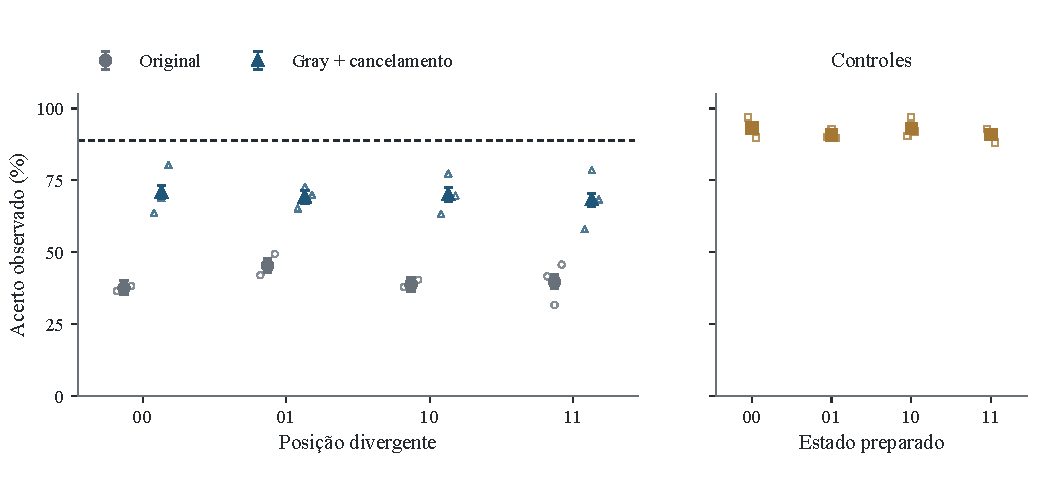
\includegraphics[width=\textwidth]{ibm-repeticoes.pdf}
\caption{Acertos na IBM. À esquerda, cada endereço indica a linha alterada. Os símbolos preenchidos reúnem as 1.536 medições de cada caso; os vazados mostram cada bloco de 512 repetições. As barras indicam a incerteza de amostragem calculada pelo intervalo de Wilson de 95\%, sem abranger toda a variação entre blocos. À direita, os controles preparam respostas conhecidas sem executar Grover. A linha tracejada de 88,89\% indica o limite de comparação com a busca clássica, aplicável somente ao painel de buscas.}
\label{fig:repeticoes}
\end{figure*}

\subsection{Descrição objetiva dos resultados}
A reconferência nacional não encontrou divergências nos registros examinados. A busca quântica usou diferenças artificiais em cópias. A versão simplificada apresentou mais acertos no modelo local e nos 12 pares de testes físicos. Na IBM, permaneceu abaixo da referência clássica na convenção de custo adotada.

\section{Discussão}
Encontrar uma diferença, explicar sua origem e demonstrar vantagem quântica são conclusões distintas. Os testes mostram que o circuito consegue localizar a linha alterada e que seu acerto muda conforme a implementação e as condições de execução. A conferência nacional, por sua vez, mostrou concordância entre os arquivos examinados. As subseções seguintes relacionam esses achados à hipótese e aos objetivos do trabalho.

\subsection{Análise das hipóteses e objetivos}
A hipótese exploratória foi sustentada nas condições definidas para a simulação. Com intensidade de ruído $\lambda=0{,}003$, o acerto da posição mais difícil passou de 83,54\% na versão original para 95,61\% com Gray e cancelamento. A comparação manteve a configuração de compilação, isto é, as regras usadas para transformar o programa nas operações executadas. Na IBM, a versão simplificada também apresentou maior acerto nos 12 pares de posição e bloco. Isso não demonstra que a simplificação explique sozinha a diferença observada na máquina, pois mudaram também os qubits físicos e a ordem dos testes.

Os quatro objetivos específicos tiveram os seguintes resultados:
\begin{enumerate}
\item A comparação nacional conferiu contagens, totais, duplicatas e presença das seções. Os registros examinados concordaram, dentro do alcance descrito na metodologia.
\item Os controles detectaram as quatro alterações conhecidas. A regra do circuito passou pelas 708 verificações locais. Esses testes dão evidência de funcionamento nos casos examinados, sem garantir ausência de qualquer erro no programa.
\item As três versões foram comparadas nas quatro posições sob as mesmas condições de simulação. A versão com Gray e cancelamento teve o maior acerto mínimo no parâmetro definido pela hipótese.
\item Os três blocos IBM permitiram medir o acerto e compará-lo com o modelo calibrado. Esse modelo previu resultados melhores do que os observados, e nenhuma busca física atingiu o limite de 88,89\%.
\end{enumerate}
Identificar quando as repetições eliminam a economia de consultas também responde à pergunta de pesquisa.

\subsection{Preparação dos dados e alcance da busca}
A redução teórica de consultas não elimina o trabalho de preparar os dados. Para construir este circuito, o programa precisa ler as duas contagens de cada linha e criar seus códigos. Nesse momento, já dispõe dos valores necessários para compará-los classicamente. Além disso, as operações que carregam os códigos são executadas a cada tentativa quântica. Mesmo o acerto ideal de 100\% não demonstra redução do trabalho completo.

A conferência nacional exige ainda verificar se alguma seção está ausente e examinar as diferenças que existirem. O teste quântico resolve uma tarefa menor: localizar uma diferença cuja existência é garantida. Quando a quantidade de diferenças é desconhecida, o procedimento e sua regra de parada precisam mudar~\cite{boyer1998}. Programas clássicos também podem dividir os arquivos entre processadores. O artigo não mediu uma vantagem de tempo sobre essa alternativa.

Para verificar se o resultado dependia apenas da alteração de um voto, uma análise já realizada usou mudanças de $-10$, $-2$, $+1$, $+10$ e $+100$ votos por posição. Foi omitido o caso que produziria contagem negativa. Nos 19 casos válidos, Gray com cancelamento apresentou maior acerto no modelo com $\lambda=0{,}003$, com diferenças de 0,24 a 12,07 pontos percentuais. Essa evidência amplia os casos testados dentro da mesma amostra; não demonstra que essa codificação seja sempre melhor.

\subsection{Comparação com trabalhos relacionados}
Stoudenmire e Waintal~\cite{stoudenmire2024} discutem o custo das operações que compõem o oráculo, a regra de reconhecimento usada por Grover. Nosso experimento apresenta um exemplo concreto dessa questão: preparar a regra exige ler contagens que já podem ser comparadas. A limitação observada pertence a esta implementação e não permite concluir que toda aplicação de Grover perde sua vantagem.

Pokharel e Lidar~\cite{pokharel2024} estudam melhorias com técnicas de detecção e redução de erros. Aqui, comparamos formas mais curtas de executar a mesma regra, sem empregar aquelas técnicas. Os percentuais de acerto não devem ser tratados como uma competição entre os trabalhos, pois os circuitos, equipamentos e critérios de comparação diferem. Na versão consultada, o estudo de Bautra e colaboradores~\cite{bautra2026} examina os limites de simulações baseadas na calibração. Nosso modelo superestimou os acertos, mostrando a necessidade de compará-lo com as medições do próprio circuito.

No campo eleitoral, Lindeman e Stark~\cite{lindeman2012} descrevem auditorias com controle estatístico do risco de confirmar um resultado incorreto. A nossa comparação entre arquivos digitais relacionados não oferece essa garantia. O resultado obtido é a concordância das contagens publicadas, dentro das verificações executadas.

\subsection{Interpretação do hardware e do controle sem diferenças}
Os testes posteriores conferiram a correspondência dos bits, isto é, se uma resposta como 01 estava sendo interpretada como a linha correta. Também permitiram observar variações entre blocos. Eles não isolaram a causa dos 16,16\% de acerto da execução inicial. Por exemplo, na versão simplificada, o acerto da posição 11 variou de 58,01\% a 78,52\%. Mudaram o momento, a ordem dos testes e os qubits escolhidos pelo compilador; não é possível atribuir essa variação a um único fator.

No controle inicial com tabelas iguais, nenhuma das 28.672 respostas foi aceita. Depois de medir qualquer endereço, a comparação clássica encontra valores iguais naquela linha e rejeita a resposta. Esse controle mostra que a verificação rejeitou as saídas quando as tabelas coincidiam. Ele não demonstra que Grover consiga provar a ausência de diferenças.

\subsection{O que a conferência permite concluir}
Uma contagem diferente entre RDV e BU, uma soma incompatível com a divulgação ou uma seção ausente pode ser apontada pelos procedimentos implementados. A concordância entre arquivos da mesma origem, porém, não exclui um erro comum aos dois. Também não mostra, por si só, que cada registro corresponde à intenção do eleitor.

As atas do Teste de Integridade trazem outra espécie de evidência: votos previamente conhecidos são comparados às saídas de urnas selecionadas. Na Câmara Legislativa do Distrito Federal, uma diferença foi atribuída, após revisão das filmagens, à digitação de 11 quando a cédula indicava branco~\cite{treDfAtaCldf2026}. A ata do TSE registrou concordância final, mas não esclareceu a causa de dois episódios chamados de falso positivo~\cite{treDfAtaTse2026}. Essas evidências são de terceiros e se limitam aos testes documentados. Elas ajudam a distinguir a detecção de uma diferença da investigação de sua causa.

\subsection{Limitações}
A parte quântica usa quatro categorias de uma única seção e diferenças artificiais. Seus resultados não representam a execução de Grover sobre a eleição inteira. Os arquivos nacionais comparados foram publicados pelo mesmo órgão; não houve confronto nacional com boletins impressos nem observação dos votos dados. A verificação da assinatura do resultado nacional também não equivale a verificar as assinaturas de todas as urnas.

A comparação de custo conta consultas e verificações com peso igual. Ela deixa de fora a leitura dos arquivos, a preparação do circuito e o tempo de execução. O protocolo de repetição descarta tentativas anteriores e não pretende ser a melhor estratégia possível. O número $2/p$ resume esse protocolo sob condições constantes, que não abrangem toda a variação observada na IBM.

O modelo calibrado trata cada teste isoladamente. Não reproduz esperas, falhas de reinicialização, influência de um teste sobre outro ou erros que ocorrem conjuntamente. Os controles também misturam preparação e leitura e podem usar qubits diferentes dos da busca. Por isso, não foram usados para corrigir as contagens. Os intervalos estatísticos apresentados descrevem a incerteza de amostragem de cada caso, sem incluir toda a variação entre blocos.

\subsection{Trabalhos futuros}
Um próximo experimento pode usar outras seções e mais posições, incluindo casos em que não se sabe se existe uma divergência. Isso exigirá adaptar a busca e estabelecer quando parar, com um limite explícito para o risco de deixar passar uma diferença.

Para avaliar utilidade prática, será necessário medir o tempo do processo inteiro, da leitura dos arquivos à verificação da resposta, e compará-lo com programas clássicos que dividem o trabalho entre processadores. Na IBM, testes com os mesmos qubits físicos e calibração próxima à execução ajudariam a separar os efeitos da implementação dos efeitos da máquina.

Uma investigação eleitoral mais ampla poderia confrontar os arquivos publicados com boletins impressos recolhidos por observadores. Essa coleta independe da divulgação online, mas o boletim continua sendo produzido pela própria urna e não comprova a intenção do eleitor. Os resultados documentados dos testes de integridade podem complementar a investigação, respeitando o alcance das urnas testadas.

\section{Organização dos códigos e dados utilizados}
O material público mantém separados os arquivos oficiais, as cópias alteradas para teste e os resultados das simulações e da IBM. O README é o arquivo de orientação: explica o conteúdo das pastas e como reproduzir as análises. O roteiro distingue reler os dados preservados de baixar novamente os arquivos nacionais.

O programa \texttt{reavaliar.py} reproduz a comparação local dos circuitos; \texttt{testar-controles.py} confere as quatro alterações no comparador clássico; e \texttt{testar-variacoes.py} reproduz os 19 casos adicionais. Já \texttt{analisar-repeticoes.py} lê as respostas exportadas da IBM e calcula as tabelas e o modelo calibrado. Analisar essas exportações não envia novos trabalhos nem consome tempo do computador quântico.

Código, dados e fontes do artigo estão em \url{https://github.com/bernardomeirelles-comp/grover-auditoria-eleitoral-2026}, versão \texttt{sprint3-final}. O manifesto de hashes, uma lista de identificadores calculados a partir dos arquivos, permite conferir a integridade das cópias. As configurações, sementes de sorteio, datas e identificadores dos trabalhos permitem relacionar cada resultado à execução que o produziu.

\section{Conclusão}
O trabalho partiu de uma pergunta concreta: as contagens dos registros de votos concordam com as dos boletins, e como localizar uma linha em que elas diferem? A conferência clássica dos 499.207 pares examinados não encontrou divergências e reproduziu os totais publicados. Esse resultado sustenta a consistência dos arquivos comparados.

Para avaliar Grover, foram introduzidas diferenças conhecidas em cópias de quatro contagens de uma seção. O circuito localizou a linha alterada na simulação ideal. Sob ruído, a versão simplificada apresentou maior acerto nos casos estudados, sustentando a hipótese exploratória nas condições definidas. Nos três blocos IBM, porém, nenhuma busca alcançou os 88,89\% necessários para empatar com a referência clássica na contagem de consultas adotada.

Assim, Grover foi aplicado à busca de inconsistências em um experimento controlado. O estudo não demonstrou benefício para a conferência completa, pois preparar os dados já permite compará-los classicamente. Também não certificou ausência de fraude. Sua contribuição é mostrar, com arquivos e resultados verificáveis, como essa aplicação foi construída, em que condições funcionou e quais conclusões os testes permitem sustentar.
